\documentclass{article}
\usepackage{amsmath, amsfonts}
\usepackage{hyperref}
\usepackage{breakurl}
\usepackage{paralist}
\usepackage{algpseudocode}
\usepackage{algorithmicx}
\usepackage{algorithm}
\usepackage{geometry}
\usepackage{multirow}
\usepackage{graphicx}
\usepackage{xspace}
\geometry{margin=1in}

\begin{document}
\title{Final Report}
\author{Yige Hu and Zhiting Zhu}
\date{}
\maketitle

% declaration of the new block
\algblock{ParFor}{EndParFor}
% customizing the new block
\algnewcommand\algorithmicparfor{\textbf{parfor}}
\algnewcommand\algorithmicpardo{\textbf{do}}
\algnewcommand\algorithmicendparfor{\textbf{end\ parfor}}
\algrenewtext{ParFor}[1]{\algorithmicparfor\ #1\ \algorithmicpardo}
\algrenewtext{EndParFor}{\algorithmicendparfor}

\newcommand{\TB}[0]{threadblock\xspace}
\newcommand{\TBs}[0]{threadblocks\xspace}
\newcommand{\SM}[0]{streaming multiprocessor\xspace}
\newcommand{\SMs}[0]{streaming multiprocessors\xspace}
\newcommand{\gcc}[0]{gcc\xspace}
\newcommand{\clang}[0]{clang\xspace}

\algnewcommand\algorithmicinput{\textbf{INPUT:}}
\algnewcommand\INPUT{\item[\algorithmicinput]}

K-means clustering is an NP-hard problem in general Euclidean space 
$\mathbb{R}^d$~\cite{k-means-euclidean},
and even for instances on a plane~\cite{k-means-plane}. 
In this report, we describe a heuristic algorithm for K-means and its 
sequential and parallel variants.
We first describe the sequential version of the algorithm, and discuss three 
different ways to parallelize it. Their computational complexity is calculated and
compared.
Then, we describe some architecture-related optimization used during
the implementation.
Finally, we evaluate the sequential implementation on CPU,
and the three parallel implementations on GPU with CUDA platform.

\section{Sequential Algorithm}
The sequential algorithm below is a heuristic algorithm which does not guarantee
a global optimal. 

\begin{algorithm}
  \caption{Sequential k-means clustering} \label{seq}
  \begin{algorithmic}[1]
    \INPUT $K$: Number of clusters; $N$: number of $d$-dimensional data points; $p$: data points. 
    \Function{seq\_k-means}{$p, N, K$}
    \State Randomly generate $K$ points as cluster centroids $c[]$
    \While {!termination\_condition }
    \For {i = 1..N}
    \For {j = 1..K}
    \For {dd = 1..d}
    \State $distance += (p(i)(dd) - c(j)(dd))^2$
    \EndFor
    \EndFor
    \State Find the nearest centroid $c_{nearest}$ for $p(i)$
    \State Assign each point to the nearest cluster centroid
    \State Accumulate $p(i)$'s coordinates
    \State Divide the accumulated coords by num\_points to get the new centroid
    \EndFor
    \EndWhile
    \EndFunction
  \end{algorithmic}
\end{algorithm}

\vspace{5mm}
\noindent
Suppose $m$ is the number of iterations in a run. \\
The complexity of this algorithm is $O(NKdm)$. 

\section{Parallel k-means clustering}
An obvious way to parallelize the algorithm is to parallelize the
parts for membership assignment and recomputation on new centroids.

There are generally two ways to compute distance between a point $p(i)$
and centroid $c(j)$. Suppose $p(i) = (p_{i1}, p_{i2}, ..., p_{id})$ 
and $c(j) = (c_{j1}, c_{j2}, ..., c_{jd})$, the squared Euclidean distance 
between point p(i) and centroid c(j) can be computed as: 
\begin{align*}
  dist^2(p(i),c(j)) &= (\vec{p_i} - \vec{c_i})^2 \\
                 &= \sum\limits_{k}^d (p_{ik} - c_{jk})^2 \numberthis \label{e1}\\
             &= \norm{\vec{p_i}}^2 - 2 \vec{p_i} \cdot \vec{c_i^T} + \norm{\vec{c_i}}^2 \\
             &= \sum\limits_{k}^d p_{ik}^2 - 2 \sum\limits_{k}^d p_{ik}*c_{jk} + \sum\limits_{k}^d c_{jk}^2 \numberthis \label{e2}
\end{align*}

This leads to two categories of parallel implementation, respectively using 
(\ref{e1}) and (\ref{e2}). Their computational complexity under the big O notation
is the same. But theoretically their number of floating point computations has a 
constant time's difference. Besides, when using (\ref{e2}), we can utilize
the cuBLAS library known as highly performant. Section~\ref{ss:pure} falls
into the first category, which intuitively uses (\ref{e1}) and implementes
a native and hand-tuned kernel. Both Section~\ref{ss:cublas} and ~\ref{ss:mix}
use (\ref{e2}). While Section~\ref{ss:cublas} uses cuBLAS library 
functions for computing both matrix inner product and vector norms, 
Section~\ref{ss:mix} implements its own vector norm function by computing the 
product of the matrix comprised by vectors, which turns out to be much 
efficient than cuBLAS's own implementation.


\subsection{Intuitive CUDA implementation}
\label{ss:pure}

One intuitive parallel implementation, which computes the distance 
using (\ref{e1}), is described as Algorithm~\ref{par}. 

\begin{algorithm}[!h]
  \caption{Parallel k-means clustering} \label{par}
  \begin{algorithmic}[1]
    \INPUT $K$: Number of clusters; $N$: number of d-dimensional data points; $p$: data points.
    \Function{par\_k-means}{$p, N, K$} \label{alg:p}
    \State Randomly choose $K$ points as cluster centroids $c[]$
    \While {! termination\_condition}
    \ParFor {i = 1..N}
    \For {j = 1..K}
    \For {dd = 1..d}
    \State $distance += (p(i)(dd) - c(j)(dd))^2$
    \EndFor
    \EndFor
    \State Find the nearest centroid $c_{nearest}$ for $p(i)$
    \State Change membership of $p(i)$ to the cluster with $c_{nearest}$
    \State Accumulate $p(i)$'s coordinates to the cluster's new centroid
    \EndParFor
    \State Compute new $c[]$: divide the accumulated coords by num\_points
    \State Recalculate termination condition
    \EndWhile
    \EndFunction  
  \end{algorithmic}
\end{algorithm}

\vspace{5mm}
\noindent
Suppose $m$ is the number of iterations in a run. The work-depth model for this algorithm is: \\
Work = $O(NKdm)$, Depth = $O(Kdm)$.



\subsection{CUDA implementation with cuBLAS}
\label{ss:cublas}

By using \ref{e2}, we can utilize two functions provided by cuBLAS.
$\norm{\vec{p_i}}$ and $\norm{\vec{c_i}}$ are calculated by \textbf{cublasSgemm()},
and $2\vec{p_i} \cdot \vec{c_i^T}$ by \textbf{cublasSnrm2()}.
Such a parallelization is shown in Algorithm~\ref{par_m}:

\begin{algorithm}[!h]
  \caption{Parallel k-means clustering using cuBLAS} \label{par_m}
  \begin{algorithmic}[1]
    \INPUT $K$: Number of clusters; $N$: number of $d$-dimensional data points; $p$: data points.
    \Function{par\_k-means-matrix}{$p, N, K$} \label{alg:pm}
    \State Randomly choose $K$ points as cluster centroids $c[]$
    \For {i = 1..N}
    \State $p\_norm^2(i) = \norm{p(i))}^2$
    \EndFor
    \While {! termination\_condition}
    \For {j = 1..K}
    \State $c\_norm^2(j) = \norm{(c(j))}^2$
    \EndFor
    \State $pc\_product = 2 p \cdot c^T$
    \ParFor {i = 1..N}
    \For {j = 1..K}
    \State $distance = p\_norm^2(i) + c\_norm^2(j) - pc\_product(i)(j)$
    \EndFor
    \State Find the nearest centroid $c_{nearest}$ for $p(i)$
    \State Change membership of $p(i)$ to the cluster with $c_{nearest}$
    \State Accumulate $p(i)$'s coordinates to the cluster's new centroid
    \EndParFor
    \State Compute new $c[]$: divide the accumulated coords by num\_points
    \State Recalculate termination condition
    \EndWhile
    \EndFunction
  \end{algorithmic}
\end{algorithm}

\vspace{5mm}
\noindent
The work-depth model for this algorithm is: \\
Work = $O(Nd + Kdm + NKdm + NKm + Ndm)$ \\
Depth = $O(D(norm(d))*N + (norm(d))*K*m + D(matrix product(NKd))*m + Km + dm)$.

\vspace{3mm}

Since we do not know the internal of cuBLAS implementions, we put place holder
in depth for algorithm~\ref{par_m}\ref{par_vn_m}. 

After the implementation, we find that it is even slower than Algorithm~\ref{par}.
Although \textbf{cublasSgemm()} is highly efficient, \textbf{cublasSnrm2()} 
turns out to be very slow, causing performance degradation.
Therefore, we implemented our own \textbf{norm\_2()} as described in 
Section~\ref{ss:mix}.


\subsection{Mixed cuBLAS with customized functions}
\label{ss:mix}

Given that there are no native cuBLAS function to collectively calculate the
sqaures of norms for each row of a matrix, and that \textbf{cublasSnrm2()} is
not performant enough, we implement our own square of norm function by utilizing
the high performant \textbf{cublasSgemm()}.
Actually, for a matrix A, the norms of each row can be got at the diagonal of 
$A * A^T$. The details are shown in Algorithm~\ref{par_vn_m}. 

\begin{algorithm}[!h]
  \caption{Parallel k-means clustering, using matrix product to compute norm} \label{par_vn_m}
  \begin{algorithmic}[1]
    \INPUT $K$: Number of clusters; $N$: number of $d$-dimensional data points; $p$: data points.
    \Function{par\_k-means-matrix-v2}{$p, N, K$} \label{alg:pm2}
    \State Randomly choose $K$ points as cluster centroids $c[]$
    \State $p\_norm\_2 = diag(p * p^T)$
    \While {! termination\_condition}
    \State $c\_norm\_2 = diag(c * c^T)$
    \State $pc\_product = 2 p \cdot c^T$
    \ParFor {i = 1..N}
    \For {j = 1..K}
    \State $distance = p\_norm\_2(i) + c\_norm\_2(j) - pc\_product(i)(j)$
    \EndFor
    \State Find the nearest centroid $c_{nearest}$ for $p(i)$
    \State Change membership of $p(i)$ to the cluster with $c_{nearest}$
    \State Accumulate $p(i)$'s coordinates to the cluster's new centroid
    \EndParFor
    \State Compute new $c[]$: divide the accumulated coords by num\_points
    \State Recalculate termination condition
    \EndWhile
    \EndFunction
  \end{algorithmic}
\end{algorithm}

\vspace{5mm}
\noindent
The work depth model for this algorithm is: \\
Work = $O(N^2dm + K^2dm + NKdm + NKm + Ndm)$, \\
Depth = $O(D(matrix product(N^2d)) + D(matrix product(K^2d)*m) + D(matrix product(NKd))*m+ Km + dm)$.

\section{Architecture-related optimizations}
\label{s:optimization}

When tuning the program performance, we use several
GPU architecture-related optimizations. Especially, coalesced memory access 
benefits the most, followed by the usage of high-speed memory regions and
prefetching.

\subsection{CUDA memory hierachy}

CUDA threads can access data from several different memory regions in GPU. Each 
thread has its own local and private memory. Each \TB has its own shared
memory regions that is accessible to all threads inside the \TB. The
global memory is large and shared by all the threads. ~\cite{cuda-program-guide}.

Per-thread-accessible registers has negligible read/write overhead compared to 
other kinds of memory access. But the total size of globally usable registers is 
fixed, and will decrease the degree of parallelism if the per \TB usage is high.
Shared memory is also a fast and restricted resource compared to global memory.
The access to the global memory is generally the slowest and dependent on the 
access pattern. A coalesced access can help achieve higher throughput
~\cite{kepler-tuning}. 

\subsection{Coalesced memory access}

For example, according to GPU's SIMD pattern, when threads in a \TB are each 
handling the computation over one single data point and tranverse over coordinates,
a column-major storage for the point matrix will enable a more coalesced global
memory access than its row-major counterpart. Therefore, we do matrix transposition
accroding to each matrix's access pattern.

Especially, in Algorithm~\ref{par_m} and ~\ref{par_vn_m}, we compute the inner 
product of the cluster centroid matrix $c$ and transposition on point matrix
$p^T$ to get a transposed version of $p \cdot c^T$, which causes coalesced memory
access in a later computational kernel without an extra matrix transposition.

\begin{align*}
  (p \cdot c^T)^T &= c \cdot p^T
\end{align*}

\subsection{High-bandwidth memory}

We load the cluster centroids into shared memory. Since centroids are sharedly 
used by computations of all threads in the kernel, spending the highly restricted
shared memory resource on them can be most beneficial. 
But for larger number of clusters with high dimensions, the shared memory
can still be not enough. In this case,
we do iterative computations over sharded input data.
We did not use the context and texture memory in this 
implemetation considering their low flexibility.

\subsection{Prefetching}

Modern C compilers like \gcc and \clang often do prefetching automatically while
compilation. CUDA platform, on the otherhand, chooses to expose more low level 
details, and rely on the developers for deciding the data access patterns. As a 
result, the CUDA C compiler is not as advanced as C compilers in optimization.
Therefore, we do manual prefetching.
This especially happens in the \textbf{dist\_square()} function in 
Algorithm~\ref{par}. In one iteration before a point coordinate is actually used, 
we load it into a thread-private register, thus overlapping loading with 
computation.

\section{Evaluation}
\subsection{Experiment platform and implementation}
We implement all algorithms in cuda and cuBlas and evaluate parallel performance on one GPU node which
has two Nvidia M2090 on TACC Lonestar. Sequential implementation is tested on CPU node with
Intel Xeon X5680 3.33GHz processor. We use one GPU to run our experiment. Nvidia M2090 is in Fermi
architecture which supports compute 2.0 capability. The peak single precision floating point performance
is 1331 GFlops. The GPU runs with CUDA 6.5 driver, 5.0
runtime library and Nvidia driver 340.32. For our implementation, we use CUDA 5.0 runtime and cublas API.
During development, we use a local GPU, Nvidia C2075 in Fermi architecture with CUDA 6.5 runtime and cuBl
as API and Nvidia driver 340.29. Peak single precision floating point performance is 1030 GFlops.
We find that our GPU code runs significant faster on our local machine than on TACC. Our GPU code
performance depends on hardware it is running on and version of CUDA API. Later version of compiler may
have optimization that results in this difference. 

\subsection{Scalability}
We evaluate the scalability of the first parallel algorithm. We cannot control how many CUDA threads it
spawns for algorithms using cuBlas library, so we just compare the performance using the same input size.
With different initial assignment of centroids, algorithms may terminate with different iterations which
impact performance measurement, so we enforce all algorithms run 50 iterations and needs to construct
120 centroids. 

\subsubsection{Strong scaling}
The input size is 640000 points with 40 dimension. Result is shown in Table~\ref{tab:strong-scaling} and
Figure~\ref{fig:strong_scaling}. 
\begin{table}[ht]
  \centering
  \begin{tabular}{|c|c|c|c|c|c|c|}
    \hline
    Number of threads	& 1000	    & 2000	    & 4000	& 8000	& 16000 & 32000\\
    \hline
    Points per thread 	&640	&320	&160	&80	&40	&20 \\
    \hline
    Time (s)	 & 71.100505	& 39.540554	& 23.712905	& 16.106382	& 14.376102	& 14.406176	\\
    \hline
  \end{tabular}
  \label{tab:strong-scaling}
  \caption{Strong scaling test for parallel algorithm~\ref{par}}
\end{table}
\begin{figure}[!h]
  \centering
  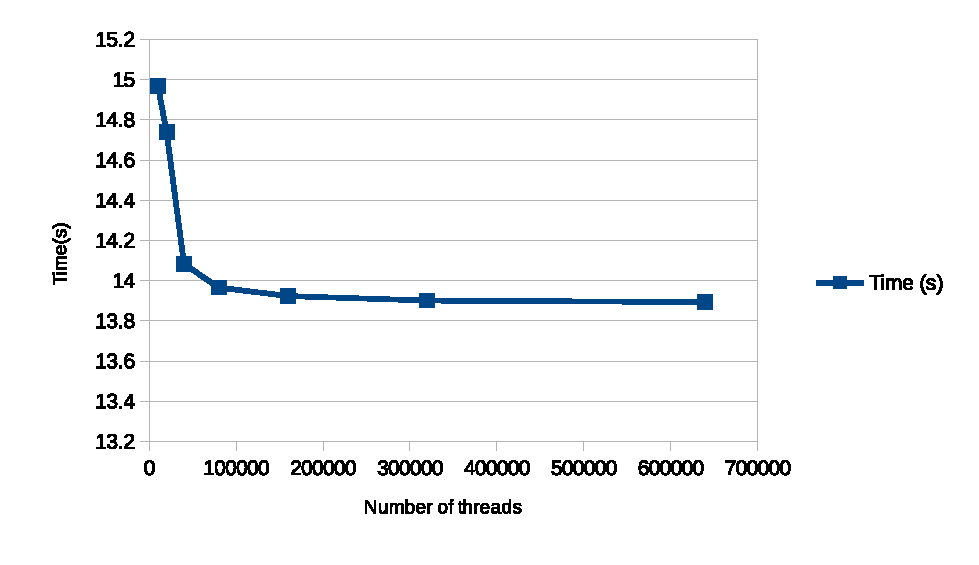
\includegraphics[width=\linewidth]{fig/strong_scaling}
  \caption{Strong scaling test for parallel algorithm~\ref{par}}
  \label{fig:strong_scaling}
\end{figure}

\subsubsection{Weak scaling}
For weak scaling, we put one point per thread. The number of points equals the total number of threads.
Result is listed in Table~\ref{tab:weak-scaling} and Figure~\ref{fig:weak_scaling}.
\begin{table}[ht]
  \centering
  \begin{tabular}{|c|c|c|c|c|c|c|}
    \hline
    Number of points	& 1000	& 2000	& 4000	& 8000	& 16000	& 32000 \\
    \hline
    Time (s)	 &4.959575	&4.995409	&4.990718	&5.086688	&5.214874	&5.493174\\
    \hline
  \end{tabular}
  \label{tab:weak-scaling}
  \caption{Weak scaling test for parallel algorithm~\ref{par}}
\end{table}
\begin{figure}[!h]
  \centering
  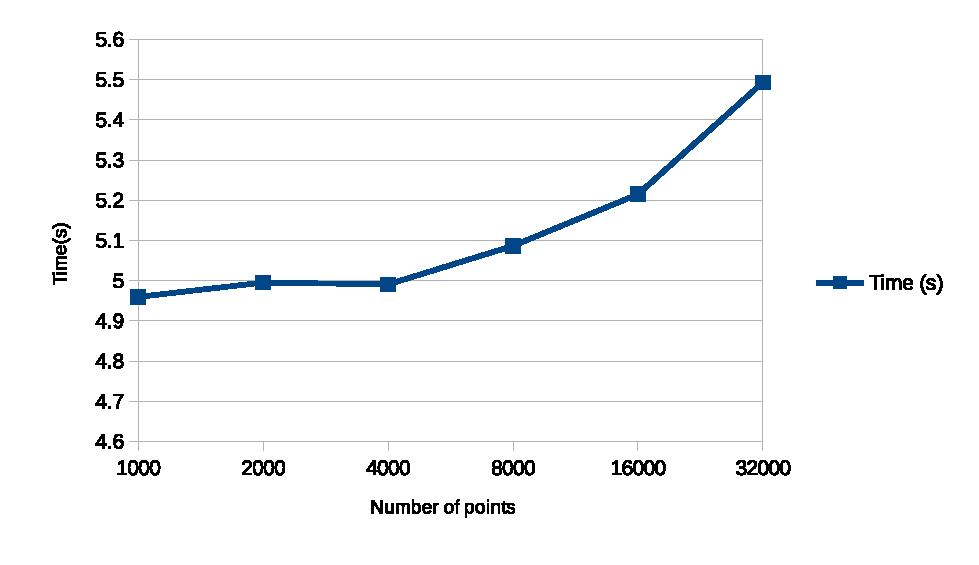
\includegraphics[width=\linewidth]{fig/weak_scaling}
  \caption{Weak scaling test for parallel algorithm~\ref{par}}
  \label{fig:weak_scaling}
\end{figure}

\subsubsection{Comparison between sequential and parallel algorithms}
We compare sequential algorithm with three versions of parallel algorithm. For each algorithm, it
receives the same input size. For the first algorithm, each thread handles one point. Result is shown in
Table~\ref{tab:comparison} and Figure~\ref{fig:all} and \ref{fig:par}. Parallel v1, v2, v3 correspond to
Algorithm~\ref{par}, \ref{par_m} and \ref{par_vn_m} respectively.   
\begin{table}[!h]
  \centering
  \begin{tabular}{|c|c|c|c|c|c|c|c|c|}
    \hline
    {}& Number of points	& 10000	& 20000	& 40000	& 80000	& 160000	& 320000	& 640000 \\
    \hline
    \multirow{4}{*}{Time(s)}	& sequential	& 13.342	& 26.397	& 52.528	& 105.078	& 210.116	& 420.287	& 840.637 \\
    \cline{2-9}
	  & parallel v1	& 5.150	& 5.335	& 5.569	& 6.213	& 7.277	& 9.324	& 13.883 \\
    \cline{2-9}
	  & parallel v2	& 5.914	& 6.603	& 7.931	& 10.267	& 15.380	& 25.137	& 44.042 \\
    \cline{2-9}
	  & parallel v3	& 5.308	& 5.559	& 6.049	& 6.932	& 8.956	& 12.662	& 20.017 \\
    \hline
  \end{tabular}
  \label{tab:comparison}
  \caption{Comparison of running time between sequential and three versions of parallel algorithms}
\end{table}

\begin{figure}[!h]
  \centering
  \begin{minipage}{.8\textwidth}
    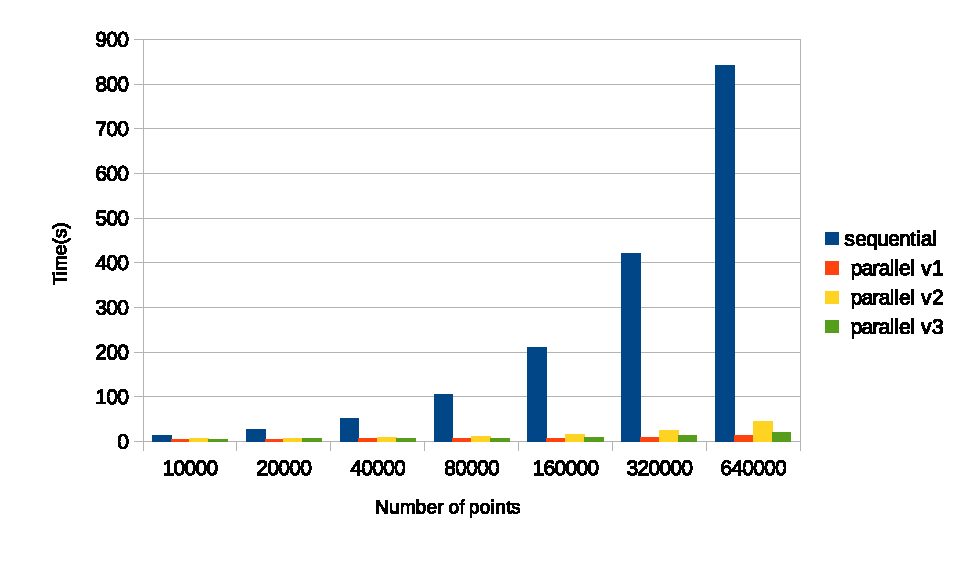
\includegraphics[width=\linewidth]{fig/all_comparison}
    \caption{Comparison of running time between sequential and three versions of parallel algorithms}
    \label{fig:all}
  \end{minipage}
  \begin{minipage}{.8\textwidth}
    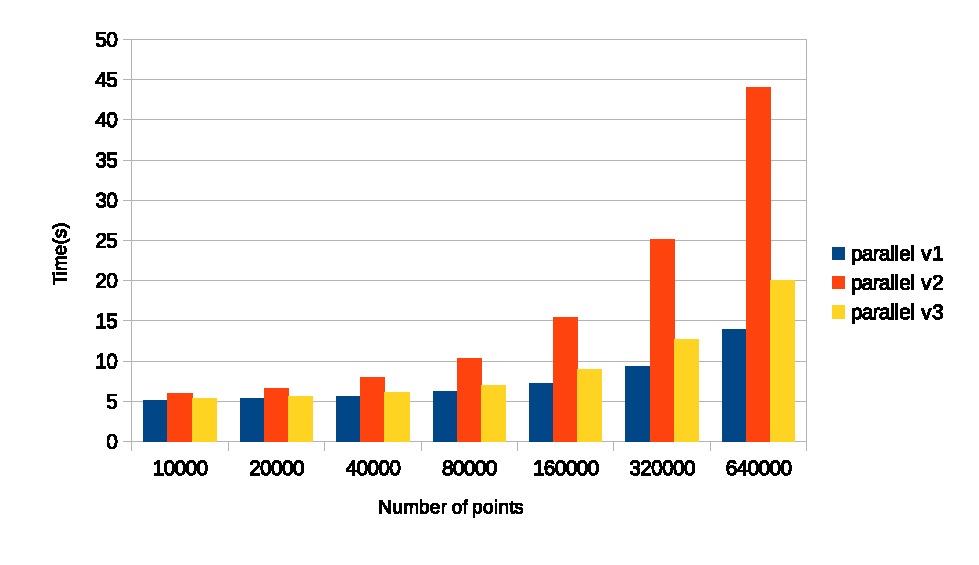
\includegraphics[width=\linewidth]{fig/parallel_algorithm_comparison}
    \caption{Comparison of three parallel algorithms}
    \label{fig:par}
  \end{minipage}
\end{figure}

From Figure~\ref{fig:par}, the hand-turned cuda implementation runs the best, followed by implementation
using cublas matrix-matrix multiplication and using matrix multiplication to calculate vector norm
and the slowest is the one using cublas snorm2 for vector norm. 

\section{Conclusion}




\bibliographystyle{acm}
\bibliography{bibliography}
\end{document}
